\section{Introduction}

The Basys2 Figure~\ref{fig:Basys2}, board is a circuit design and implementation platform that anyone can use to gain experience building real digital circuits. Built around a Xilinx Spartan-3E Field Programmable Gate Array and a Atmel AT90USB2 USB controller, the Basys2 board provides complete, ready-to-use hardware suitable for hosting circuits ranging from basic logic devices to complex controllers.


\begin{figure}[!htbp]
    \centerline{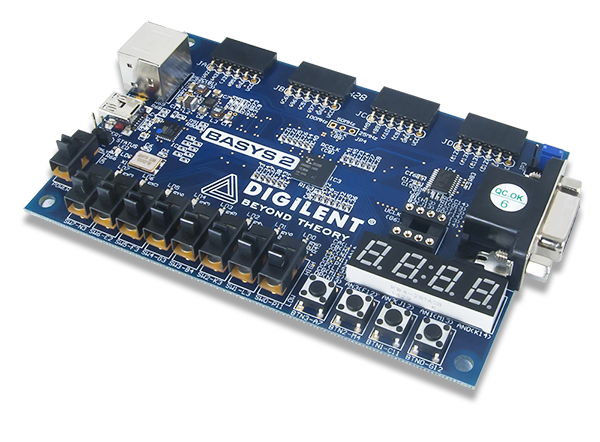
\includegraphics[width=\textwidth]{basys2-0}}
    \vspace{0cm}\caption{Basys 2 board}
    \label{fig:Basys2}
\end{figure}


Our project uses the Basys2 to make a clock with some features. We propose to use 7 segment dislay as output and the push buttons to set the time and navigate through the menus.

\noindent

